\chapter{Selective Uncertainty, Quiet-Apnea Safety, and Finite-\texorpdfstring{$K$}{K} Conformal Audit}
\label{ch:uncertainty_conformal}

\section{Motivation and evaluation scope}

Chapter~4 established R2e as the strongest internally supported candidate in the present evaluation, while showing that its gain over simpler R1a is not sufficiently robust to support a claim of general superiority. Neither result is a clinical validation. This chapter asks whether an estimator can identify unreliable predictions, abstain selectively without disproportionately suppressing quiet-apnea windows, and produce prediction intervals whose finite-sample limits are explicit.

The Stage~3 uncertainty and conformal audit (\texttt{WP3}/\texttt{WP4}) uses the frozen \texttt{pool30\_sync} cohort: 28 synchronous sessions from 11 infants. The primary waveform reference is the 1~Hz monitor-training reference; the shared Trig~$-10$~s blind sensitivity analysis follows Chapter~4. Windows are repeated observations nested within sessions and infants. Window-level summaries are descriptive; patient-level comparisons are more relevant to consistency across infants. This small internal cohort is not an external clinical validation set.

\section{Uncertainty scores and selective prediction}
\label{sec:ch5_selective}

\subsection{Scores and operating rule}

The eight proxies are U1, posterior entropy; U2, posterior standard deviation; U3, clean-waveform spectral entropy; U4, raw-waveform spectral entropy; U5, harmonic deficit; U6a, additive signal-quality index (SQI); U6b, geometric SQI; and U6c, a five-parameter SQI calibrated under leave-one-patient-out (LOPO) evaluation. U1--U5 are parameter-free scores. U6a is a fixed additive combination of normalized posterior standard deviation, posterior entropy, and the OOD barrier (weights 0.45, 0.35, and 0.20); U6b combines the same components through an equal-exponent geometric confidence score. Specifically, with $u_1 \in [0,1]$ denoting normalized posterior Shannon entropy, $u_2 \in [0,1]$ posterior standard deviation normalized by the standard deviation of the uniform 1~bpm respiratory-rate grid and clipped to $[0,1]$, and $h_{\mathrm{mix}}$ causal temporal mixture spectral entropy, the barrier is $b_{\mathrm{ood}}=\operatorname{clip}((h_{\mathrm{mix}}-\tau_{\mathrm{ood}})/(1-\tau_{\mathrm{ood}}),0,1)$. The uncertainty scores are $u_{6a}=\operatorname{clip}(0.45u_2+0.35u_1+0.20b_{\mathrm{ood}},0,1)$ and $u_{6b}=1-\big[(1-u_2)(1-u_1)(1-b_{\mathrm{ood}})\big]^{1/3}$. The weights and exponents are not fitted, but both composites use the fixed $\tau_{\mathrm{ood}}=0.90$ and a three-hop (6~s) causal history. The cutoff and history rule are design choices, so the composites are not threshold-free. U6c fits five simplex-normalized non-negative weights over U1--U5 via regularized non-negative least squares with training-fold standardization. U2 provides a simple posterior-spread reference without fitted parameters or an additional OOD barrier cutoff.

Selective prediction ranks windows from least to most uncertain, retains the lower-uncertainty fraction, and rejects the rest. Coverage, $\covLevel$, is swept from 0.50 to 1.00. Risk is RMSE among retained windows. Excess area under the risk--coverage curve ($\eaurcMetric$) is normalized by the 0.50 coverage span and measured relative to the constant random-abstention (full-coverage) baseline rather than the oracle; a negative value therefore indicates lower average risk than full coverage in bpm under this convention. The 80\% point is reported separately as a concrete operating point.

At 1~Hz, U2 yielded E-AURC $-0.2454$ [$-0.4069,-0.1168$]. At 80\% coverage, RMSE changed from 6.8486 to 6.6890~bpm, and 10 of 11 infants had lower patient-level risk. The raw patient-level comparison was $p=0.0098$; after Holm correction it was $p=0.0781$. For Trig~$-10$~s, U2 yielded E-AURC $-0.2929$ [$-0.4555,-0.1436$], and RMSE changed from 8.0634 to 7.8798~bpm. Nine of 11 infants improved; raw $p=0.0244$ and Holm-adjusted $p=0.1953$. Point estimates favor U2, but neither comparison remains statistically significant after the reported multiplicity correction.

Across all eight proxies, session-level RMSE decreased at the 80\% operating point, but the patient-level evidence was weaker: no patient-level comparison remained significant after Holm correction. Several spectral and harmonic E-AURC intervals include zero, and U6c's 1~Hz interval includes zero as well. Table~\ref{tab:ch5_selective_results} gives the complete proxy-by-reference results, and Figure~\ref{fig:ch5_risk_coverage_safety} summarizes the selective risk--coverage and pause-safety trade-off; U6c also fails the pause-safety criterion described below.

\begin{table}[htbp]
\centering
\scriptsize
\setlength{\tabcolsep}{4pt}
\caption{Selective-prediction results for all eight R2e uncertainty proxies. RMSE is the session-macro risk at full and 80\% coverage; E-AURC is the session-level area difference in bpm with its 95\% CI in brackets. Infant counts are patient-level wins for the reference shown in that column. Patient-level $p$-values are shown as raw/Holm-adjusted across the eight proxies within each reference.}
\label{tab:ch5_selective_results}
\begin{tabularx}{\textwidth}{@{}>{\raggedright\arraybackslash}p{0.8cm}>{\raggedright\arraybackslash}p{2.35cm}>{\raggedright\arraybackslash}X >{\raggedright\arraybackslash}X@{}}
\toprule
Proxy & Score & 1~Hz monitor-training reference & Trig~$-10$~s sensitivity \\
\midrule
U1 & Posterior entropy & RMSE $6.8486 \rightarrow 6.6230$~bpm; E-AURC $-0.2194$ [$-0.4015,-0.0742$]; 9/11 improved; $p=0.0244$, Holm $=0.1709$ & RMSE $8.0634 \rightarrow 7.7841$~bpm; E-AURC $-0.2530$ [$-0.4175,-0.1152$]; 9/11 improved; $p=0.1016$, Holm $=0.6094$ \\
\addlinespace[2pt]
U2 & Posterior SD & RMSE $6.8486 \rightarrow 6.6890$~bpm; E-AURC $-0.2454$ [$-0.4069,-0.1168$]; 10/11 improved; $p=0.0098$, Holm $=0.0781$ & RMSE $8.0634 \rightarrow 7.8798$~bpm; E-AURC $-0.2929$ [$-0.4555,-0.1436$]; 9/11 improved; $p=0.0244$, Holm $=0.1953$ \\
\addlinespace[2pt]
U3 & Clean spectral entropy & RMSE $6.8486 \rightarrow 6.6782$~bpm; E-AURC $-0.1776$ [$-0.5126,+0.1624$]; 8/11 improved; $p=0.2783$, Holm $=1.0000$ & RMSE $8.0634 \rightarrow 7.7517$~bpm; E-AURC $-0.3735$ [$-0.7584,+0.0533$]; 9/11 improved; $p=0.2061$, Holm $=0.6152$ \\
\addlinespace[2pt]
U4 & Raw spectral entropy & RMSE $6.8486 \rightarrow 6.6637$~bpm; E-AURC $-0.1946$ [$-0.4495,+0.1038$]; 9/11 improved; $p=0.2783$, Holm $=1.0000$ & RMSE $8.0634 \rightarrow 7.7150$~bpm; E-AURC $-0.3604$ [$-0.7117,+0.0341$]; 7/11 improved; $p=0.2061$, Holm $=0.6152$ \\
\addlinespace[2pt]
U5 & Harmonic deficit & RMSE $6.8486 \rightarrow 6.6544$~bpm; E-AURC $-0.2284$ [$-0.5454,+0.0453$]; 8/11 improved; $p=0.2402$, Holm $=1.0000$ & RMSE $8.0634 \rightarrow 7.7899$~bpm; E-AURC $-0.3752$ [$-0.6950,-0.0570$]; 8/11 improved; $p=0.1230$, Holm $=0.6152$ \\
\addlinespace[2pt]
U6a & Additive SQI & RMSE $6.8486 \rightarrow 6.5920$~bpm; E-AURC $-0.2448$ [$-0.4842,-0.0496$]; 8/11 improved; $p=0.0830$, Holm $=0.4980$ & RMSE $8.0634 \rightarrow 7.7694$~bpm; E-AURC $-0.3009$ [$-0.5284,-0.1014$]; 9/11 improved; $p=0.0830$, Holm $=0.5811$ \\
\addlinespace[2pt]
U6b & Geometric SQI & RMSE $6.8486 \rightarrow 6.5956$~bpm; E-AURC $-0.2398$ [$-0.4982,-0.0257$]; 8/11 improved; $p=0.2402$, Holm $=1.0000$ & RMSE $8.0634 \rightarrow 7.7569$~bpm; E-AURC $-0.2932$ [$-0.5500,-0.0699$]; 8/11 improved; $p=0.1230$, Holm $=0.6152$ \\
\addlinespace[2pt]
U6c & Five-parameter SQI & RMSE $6.8486 \rightarrow 6.6145$~bpm; E-AURC $-0.2688$ [$-0.5926,+0.0266$]; 8/11 improved; $p=0.2402$, Holm $=1.0000$ & RMSE $8.0634 \rightarrow 7.6774$~bpm; E-AURC $-0.4218$ [$-0.7514,-0.0828$]; 8/11 improved; $p=0.1230$, Holm $=0.6152$ \\
\bottomrule
\end{tabularx}
\end{table}

The HQI coding audit qualifies U5. In the implemented harmonic-quality calculation, the fundamental-peak bins ($\pm 2$~bpm around the fundamental peak) are included inside both the peak-plus-harmonic numerator term and the total-passband denominator term, double-counting those bins in the denominator and compressing raw values below $0.5$. The observed HQI range was [0.0655, 0.4351], versus [0.0700, 0.7193] under non-overlapping accounting. Rank ordering was nearly identical (Spearman $\rho=0.999945$), and U5's 1~Hz E-AURC on R2e changed by only $+0.0032$~bpm (from $-0.2284$ to $-0.2253$~bpm). This sensitivity result shows little change in ranking for this cohort; it does not make the definitions interchangeable.

Sequence-level future-window perturbations produced zero output difference for all eight proxies in the tested implementation. This does not establish zero end-to-end latency: the H0 front end retains a 3~s short-time Fourier transform look-ahead, as described in Chapter~4. The result therefore does not establish a fully causal, zero-look-ahead system.

\begin{figure}[htbp]
\centering
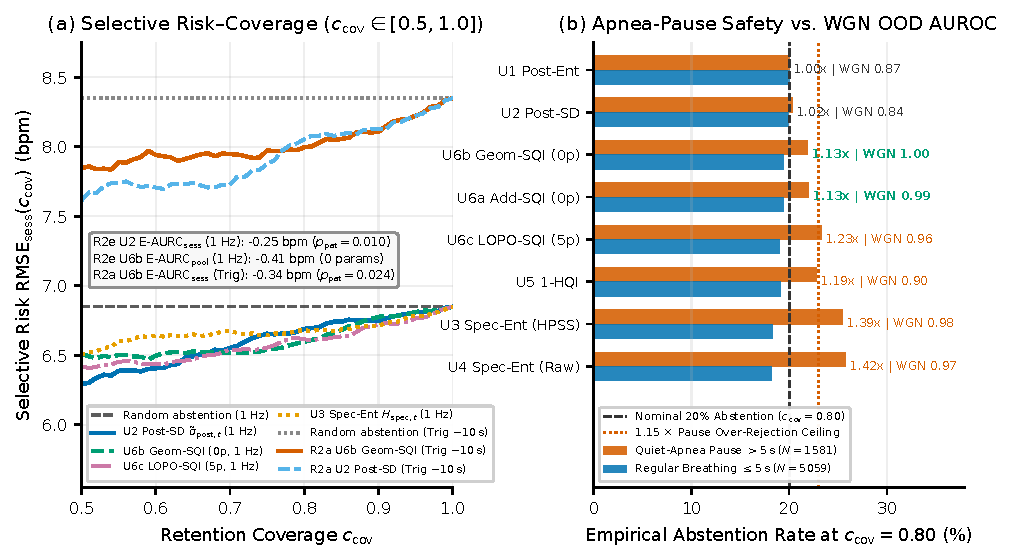
\includegraphics[width=0.95\textwidth]{stage3_risk_coverage_and_apnea_safety}
\caption{Frozen Stage~3 risk--coverage and apnea-safety summary. Panel~(a) plots equal-session selective risk $\rmseSess(\covLevel)$ for R2e on the 1~Hz reference alongside overlaid R2a curves on the lag-adjusted trigger sensitivity (\texttt{Trig~$-10$~s}); the frozen legend shorthand ``(0p)'' / ``0~params'' on U6a and U6b denotes zero fitted weights (with fixed $\tau_{\mathrm{ood}}=0.90$ and 3-hop history). Panel~(b) compares R2e pooled abstention rates at $\covLevel=0.80$ in pause ($>5$~s, $N=1{,}581$) versus regular ($\le 5$~s, $N=5{,}059$) windows alongside WGN OOD AUROC.}
\label{fig:ch5_risk_coverage_safety}
\end{figure}

\section{Quiet-apnea safety and OOD detection}
\label{sec:ch5_safety}

The pause-safety audit included 1,581 pause windows and 5,059 regular windows; pause windows were identified by an inter-breath gap greater than 5.0~s. These operational strata are not clinically adjudicated apnea events. At 80\% overall coverage, pause rejection ratio is the rejection rate among pause windows divided by the rejection rate among regular windows. The project's diagnostic limit is a ratio no greater than 1.15. This is an internal engineering criterion, not a clinical threshold.

U2 had a pause-rejection ratio of 1.0200 under global pooled 80\% thresholding and 1.0645 under within-session 80\% thresholding (pooled across sessions after per-session ranking). Its WGN OOD AUROC was 0.8406, with a false-positive rate (FPR) of 0.4515 at 95\% true-positive rate (TPR). Table~\ref{tab:ch5_pause_ood} shows the central trade-off across all eight proxies: a score can detect synthetic noise strongly while also rejecting pause windows more often.

\begin{table}[htbp]
\centering
\footnotesize
\caption{Pause-safety and synthetic WGN OOD audit for all eight R2e uncertainty proxies at 80\% overall coverage. Pause ratio reports global-threshold (pooled) / within-session-threshold rejection risk ratios (diagnostic ceiling $\le 1.15$).}
\label{tab:ch5_pause_ood}
\begin{tabularx}{\textwidth}{@{}>{\raggedright\arraybackslash}Xrrr@{}}
\toprule
Proxy & Pause rejection ratio (pool / sess) & WGN AUROC & WGN FPR at 95\% TPR \\
\midrule
U1 posterior entropy & 0.9992 / 1.0432 & 0.8698 & 0.4407 \\
U2 posterior SD & 1.0200 / 1.0645 & 0.8406 & 0.4515 \\
U3 clean spectral entropy & 1.3941 / 1.1342 & 0.9796 & 0.0926 \\
U4 raw spectral entropy & 1.4191 / 1.2292 & 0.9735 & 0.1014 \\
U5 harmonic deficit & 1.1946 / 1.1971 & 0.8982 & 0.2714 \\
U6a additive SQI & 1.1319 / 1.1122 & 0.9935 & 0.0191 \\
U6b geometric SQI & 1.1275 / 1.1209 & 0.9986 & 0.0036 \\
U6c calibrated SQI & 1.2266 / 1.1971 & 0.9635 & 0.1209 \\
\bottomrule
\end{tabularx}
\end{table}

At the selected $\tau_{\mathrm{ood}}=0.90$ with three-hop history, U6b met the project's pause-ratio limit and separated the tested WGN condition (AUROC 0.9986; FPR 0.0036 at 95\% TPR). The audit also recorded no barrier triggers for the tested synthetic shallow-breathing conditions down to 0.2~mm and 10~dB (28, 45, and 75~bpm). In auxiliary targeted non-child (UCD) audits, blind waveform-only U6b reached AUROC 0.6235 across all 261 partial-window ($>0\%$) non-child windows and AUROC 0.9055 on the 32 majority-corrupted ($\ge 50\%$) windows, whereas deterministic firmware telemetry gating yielded AUROC 1.0. The Stage~3 invariance check on H5 reported a maximum numerical difference of $8.88\times10^{-16}$ under the tested $O(2)\times\mathbb{R}_{>0}$ transformations; on the primary H0-backed R2e path, post-freeze fuzzing verified $SO(2)\times\mathbb{R}_{>0}$ invariance to $\le 2.22\times10^{-16}$ for U6b alongside an I/Q-swap Nyquist clamping residual of $\le 5.24\times10^{-6}$. These results concern specified synthetic or targeted audit conditions; they do not validate performance across external hospitals, devices, patient populations, or naturally occurring failure modes.

Table~\ref{tab:ch5_u6b_sensitivity} reports the full tested cutoff and history sensitivity for U6b. The pooled pause ratio is evaluated at 80\% coverage; patient wins and $p$-values are for the 1~Hz selective-risk comparison. These raw $p$-values are not adjusted across the cutoff and history configurations and are exploratory.

\begin{table}[htbp]
\centering
\footnotesize
\caption{U6b cutoff and history sensitivity on R2e. E-AURC is in bpm; pause ratio is pooled at 80\% coverage. WGN results are AUROC and FPR at 95\% TPR. ``None'' means no entropy cutoff ($b_{\mathrm{ood}}=h_{\mathrm{mix}}$). Patient $p$-values are raw and unadjusted across configurations.}
\label{tab:ch5_u6b_sensitivity}
\begin{tabularx}{\textwidth}{@{}cc>{\raggedright\arraybackslash}Xrr@{}}
\toprule
History hops & $\tau_{\mathrm{ood}}$ & E-AURC; wins; raw patient $p$ & Pause ratio & WGN AUROC / FPR \\
\midrule
3 & None & $-0.2396$; 8/11; 0.3203 & 1.3160 (fail) & 0.9990 / 0.0030 \\
3 & 0.75 & $-0.2365$; 8/11; 0.3203 & 1.3160 (fail) & 0.9990 / 0.0030 \\
3 & 0.80 & $-0.2307$; 8/11; 0.3203 & 1.3160 (fail) & 0.9990 / 0.0030 \\
3 & 0.85 & $-0.2308$; 8/11; 0.3203 & 1.3016 (fail) & 0.9990 / 0.0030 \\
3 & 0.88 & $-0.2424$; 8/11; 0.2783 & 1.1765 (fail) & 0.9989 / 0.0030 \\
3 & 0.90 (locked) & $-0.2398$; 8/11; 0.2402 & 1.1275 (pass) & 0.9986 / 0.0036 \\
3 & 0.92 & $-0.2282$; 9/11; 0.0322 & 1.0284 (pass) & 0.9968 / 0.0075 \\
3 & 0.95 & $-0.2194$; 9/11; 0.0244 & 1.0075 (pass) & 0.9482 / 0.2444 \\
0 & 0.90 & $-0.2329$; 9/11; 0.0420 & 1.0666 (pass) & 0.9509 / 0.1645 \\
1 & 0.90 & $-0.2376$; 8/11; 0.0830 & 1.1099 (pass) & 0.9955 / 0.0139 \\
2 & 0.90 & $-0.2403$; 8/11; 0.1230 & 1.1275 (pass) & 0.9979 / 0.0060 \\
5 & 0.90 & $-0.2240$; 8/11; 0.4131 & 1.1275 (pass) & 0.9989 / 0.0018 \\
\bottomrule
\end{tabularx}
\end{table}

Among the listed three-hop cutoff points, 0.90 and 0.92 met both the pause ratio limit and the project's WGN AUROC criterion of 0.95. At 0.95, pause rejection was lowest but WGN AUROC fell below 0.95. Cutoffs of 0.88 and below failed the pause limit despite strong WGN detection. At $\tau_{\mathrm{ood}}=0.90$, all tested histories (0, 1, 2, 3, and 5 hops) met both project criteria; the zero-hop AUROC of 0.9509 was only marginally above the threshold. This supports reporting the locked three-hop setting as a measured operating point, not as a universally optimal cutoff.

This is the pause-safety/OOD trade-off in the present evaluation. Lowering the barrier cutoff increases rejection of high-entropy windows: that strengthens WGN detection but can reject quiet breathing pauses disproportionately. A plausible signal-level explanation is that a pause weakens periodic harmonic structure and can make the normalized spectrum flatter, raising spectral entropy; this is an interpretation of the observed score behavior, not a clinical characterization of the pauses. At three-hop history, the NICU causal temporal mixture spectral-entropy 95th percentile was 0.9130, compared with 0.9498 at the WGN 5th percentile. Their proximity makes the operating point sensitive to threshold choice. U6b at 0.90 is an empirically selected, data-motivated cutoff for this cohort and these audits. It is not threshold-free or a universally safe setting. U6c's pause ratio of 1.2266 exceeds the project's 1.15 limit despite favorable risk--coverage point estimates.

\section{Finite-\texorpdfstring{$K$}{K} conformal calibration}
\label{sec:ch5_conformal}

\subsection{Calibration units and finite-rank limit}

Each LOPO fold has $K_{\mathrm{cal}}=10$ calibration patients because one of the 11 infants is held out. For a split-conformal order statistic at miscoverage level $\alpha$, the finite-sample rank is
\[
i_{\alpha}=\left\lceil (K_{\mathrm{cal}}+1)(1-\alpha)\right\rceil.
\]
At a nominal 95\% target, $\alpha=0.05$ and $i_{\alpha}=\lceil 11(0.95)\rceil=11$, which exceeds the ten available calibration patients. Thus the patient-level C4 and C5 intervals are infinite (vacuous) at this target. C1--C3 return finite intervals by using window- or session-level calibration units, but those constructions do not provide the same patient-level exchangeability basis. With ten calibration patients, the smallest nonzero attainable tail probability is $1/(K_{\mathrm{cal}}+1)=1/11\approx0.0909$. At least 19 calibration patients are needed for this rank construction to return a finite patient-level interval at a 95\% target.

This is a resolution limit imposed by the number of independent calibration units. Adding windows from the same infants does not create more independent patients. The audit compared five constructions:
\begin{itemize}
\item C1 randomly splits windows 50/50 between calibration and evaluation. Windows from the same patients may enter both partitions, creating patient-level leakage.
\item C2 uses LOPO but treats pooled windows as exchangeability units. Repeated windows from an infant are correlated, so this unit does not match the data structure.
\item C3 computes within-session quantiles and an outer session-level order statistic, using sessions as calibration units even though multiple sessions remain clustered within patients.
\item C4 first computes within-patient absolute-error quantiles and then applies an outer patient-level quantile.
\item C5 follows the same two-level structure after scaling absolute error by posterior standard deviation floored at 1~bpm, then rescales the calibrated radius.
\end{itemize}

C4 and C5 are local two-level patient-quantile procedures motivated by hierarchical conformal work. They do not automatically inherit a theorem that guarantees distribution-free coverage for this cohort. When the same nominal level is used at both levels, the simple hierarchical bound is $(1-\alpha)^2$, rather than $1-\alpha$, under the required hierarchical assumptions. In Dunn et al.'s supervised new-group setting, CDF pooling is asymptotically valid for continuous outcomes, single subsampling has finite-sample $1-\alpha$ validity, and repeated subsampling (aggregating $p$-values into a single set) has a finite-sample $1-2\alpha$ lower bound \citep{dunn2023distribution}. The head-to-head table evaluates Dunn et al.'s CDF-pooling rule and a $B=200$ Monte Carlo average of single-draw subsampling (replicating single-draw subsampling 200 times and averaging coverage and width rather than constructing a $p$-value-averaged repeated-subsampling set); empirical averages here should not be confused with a finite-sample guarantee on our cohort. Dunn's guarantees also rely on the relevant within-group and between-group exchangeability assumptions. Our 30~s windows overlap by 93.3\% and are serially dependent, so these methods are empirical comparators here; no distribution-free guarantee is claimed for their local use or for C4/C5.

\subsection{Empirical coverage across target levels}

Table~\ref{tab:ch5_conformal_all} and Figure~\ref{fig:ch5_finite_k_conformal} report frozen R2e LOPO results for the 1~Hz monitor-training reference. Mean and minimum coverage are calculated across the 11 held-out patients; undercovered counts patients below the nominal target. Pooled coverage and mean full interval width show how aggregate behavior can differ from patient-level behavior. At the 95\% target, C4 and C5 return vacuous intervals, so their empirical coverage is 1 and their mean width is infinite. The other values are empirical outcomes on this cohort, not guarantees for future infants.

\begin{table}[htbp]
\centering
\footnotesize
\setlength{\tabcolsep}{4pt}
\caption{R2e LOPO conformal audit for the 1~Hz monitor-training reference by nominal coverage target. Width is mean full interval width in bpm. C4 and C5 are vacuous at the 95\% target because the finite-sample rank is unavailable.}
\label{tab:ch5_conformal_all}
\begin{tabularx}{\textwidth}{@{}cc>{\raggedleft\arraybackslash}Xrrrr@{}}
\toprule
Method & Target & Mean patient cov & Minimum & Undercovered & Pooled cov & Mean width \\
\midrule
C1 & 0.95 & 0.933 & 0.789 & 5 & 0.947 & 29.12 \\
C2 & 0.95 & 0.934 & 0.785 & 4 & 0.946 & 29.32 \\
C3 & 0.95 & 0.995 & 0.968 & 0 & 0.995 & 50.60 \\
C4 & 0.95 & 1.000 & 1.000 & 0 & 1.000 & $\infty$ \\
C5 & 0.95 & 1.000 & 1.000 & 0 & 1.000 & $\infty$ \\
\midrule
C1 & 0.90 & 0.892 & 0.677 & 4 & 0.909 & 23.62 \\
C2 & 0.90 & 0.881 & 0.623 & 4 & 0.898 & 23.23 \\
C3 & 0.90 & 0.975 & 0.875 & 1 & 0.978 & 38.51 \\
C4 & 0.90 & 0.976 & 0.875 & 1 & 0.979 & 38.84 \\
C5 & 0.90 & 0.963 & 0.847 & 1 & 0.970 & 39.18 \\
\midrule
C1 & 0.80 & 0.798 & 0.477 & 5 & 0.812 & 17.30 \\
C2 & 0.80 & 0.772 & 0.398 & 5 & 0.795 & 17.00 \\
C3 & 0.80 & 0.885 & 0.632 & 2 & 0.904 & 23.83 \\
C4 & 0.80 & 0.895 & 0.551 & 2 & 0.919 & 25.57 \\
C5 & 0.80 & 0.864 & 0.586 & 2 & 0.881 & 24.02 \\
\midrule
C1 & 0.70 & 0.692 & 0.350 & 6 & 0.703 & 13.14 \\
C2 & 0.70 & 0.677 & 0.292 & 5 & 0.697 & 13.09 \\
C3 & 0.70 & 0.758 & 0.366 & 4 & 0.780 & 16.41 \\
C4 & 0.70 & 0.760 & 0.389 & 3 & 0.783 & 16.27 \\
C5 & 0.70 & 0.766 & 0.440 & 3 & 0.777 & 17.62 \\
\bottomrule
\end{tabularx}
\end{table}

At the 80\% target, C1 pooled coverage is 0.812 while its minimum patient coverage is 0.477; C2 pooled coverage is 0.795 and minimum patient coverage is 0.398. Pooled or cohort averages therefore do not describe how intervals behave for every infant. C3--C5 have higher mean patient coverage at this target, but minimum patient coverage remains between 0.551 and 0.632, and their intervals are wider than C1 and C2. At the 70\% target, all methods show substantial patient-to-patient variation; C5's mean coverage of 0.766 accompanies a minimum of 0.440.

For C5 at the 80\% target, mean full interval width was 17.96~bpm in the within-patient median-split low-posterior-SD half and 30.54~bpm in the high-posterior-SD half. These are full interval widths ($2\hat{q}\tilde{\sigma}$), not half-widths. Scaling adapts interval size to posterior uncertainty but does not resolve the finite-rank limit or provide nominal per-infant guarantees.

\begin{figure}[htbp]
\centering
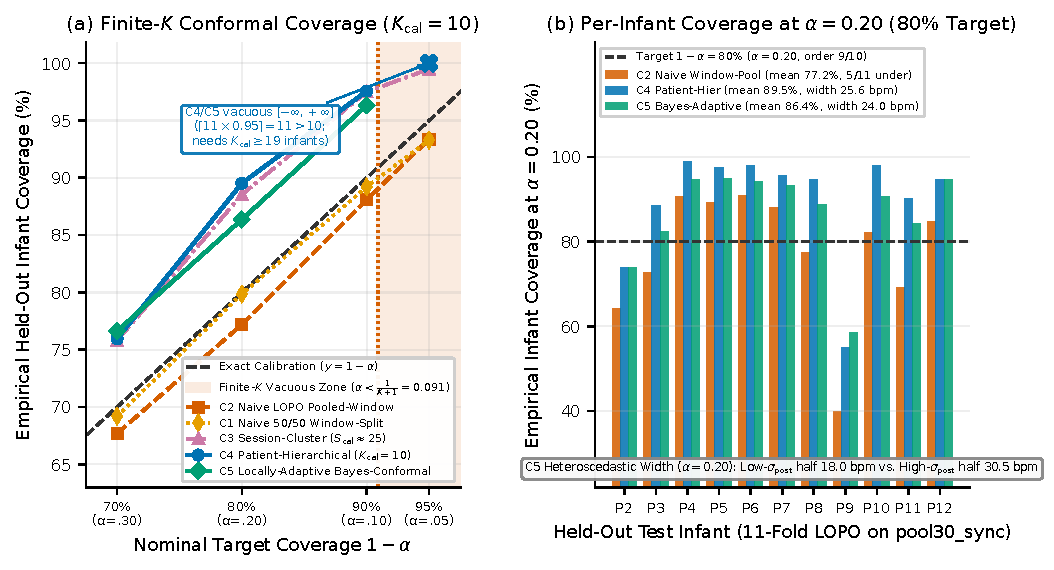
\includegraphics[width=0.95\textwidth]{stage3_finite_k_conformal_audit}
\caption{Frozen Stage~3 finite-$K$ conformal audit on R2e (1~Hz reference). Panel~(a) plots mean held-out infant coverage across nominal targets ($70\%$--$95\%$), marking the finite-$K$ vacuous zone ($\alpha < 1/(K_{\mathrm{cal}}+1)=0.091$) and vacuous 95\% C4/C5 intervals. Panel~(b) shows per-infant coverage across all 11 held-out infants at the 80\% target ($\alpha=0.20$) for C2, C4, and C5; in the embedded C5 callout, ``half'' denotes the within-patient median-split low-/high-$\sigma_{\mathrm{post}}$ window halves, and $18.0$/$30.5$~bpm are full interval widths, not half-widths.}
\label{fig:ch5_finite_k_conformal}
\end{figure}

\subsection{Head-to-head comparison with hierarchical methods}

The R2e 1~Hz head-to-head results are summarized in Table~\ref{tab:ch5_dunn_comparison}. At the 95\% target, the patient-level two-layer methods and the Dunn comparisons are all vacuous with ten calibration patients per fold. At the lower targets, CDF pooling generally has higher empirical patient coverage and larger intervals than the $B=200$ Monte Carlo single-draw subsampling average; C5 trades coverage against interval width differently. These are empirical comparisons across 11 held-out infants, not a universal ranking or a transfer of Dunn et al.'s guarantee to C4/C5.

\begin{table}[htbp]
\centering
\footnotesize
\setlength{\tabcolsep}{4pt}
\caption{R2e patient-level head-to-head conformal audit on the 1~Hz reference. Undercovered is the number of infants below target out of 11. Width is mean full interval width in bpm; bracketed values are within-patient median-split low-/high-posterior-SD full widths. The subsampling rows report the $B=200$ Monte Carlo average of single-draw subsampling. The 95\% row is vacuous for all listed methods; the 70\% block reports adaptive rows only (subgroup widths omitted).}
\label{tab:ch5_dunn_comparison}
\begin{tabularx}{\textwidth}{@{}c l >{\raggedright\arraybackslash}X r r@{}}
\toprule
Target & Form & Method & Mean / min cov; under & Mean width \\
\midrule
0.95 & All & C4, C5, Dunn CDF pooling, and single-draw subsampling ($B=200$ MC avg.) & 1.000 / 1.000; 0/11 & $\infty$ \\
\midrule
0.90 & Unweighted & C4 & 0.9756 / 0.8750; 1/11 & 38.84 \\
0.90 & Unweighted & Dunn CDF pooling & 0.9874 / 0.9144; 0/11 & 44.26 \\
0.90 & Unweighted & Dunn single-draw subsampling ($B=200$ MC avg.) & 0.9083 / 0.7020; 4/11 & 30.61 \\
0.90 & Adaptive & C5 & 0.9632 / 0.8472; 1/11 & 39.18 [29.30 / 49.82] \\
0.90 & Adaptive & Dunn CDF pooling & 0.9880 / 0.9213; 0/11 & 52.82 [39.51 / 67.17] \\
0.90 & Adaptive & Dunn single-draw subsampling ($B=200$ MC avg.) & 0.9056 / 0.7010; 4/11 & 33.83 [25.35 / 43.01] \\
\midrule
0.80 & Unweighted & C4 & 0.8952 / 0.5509; 2/11 & 25.57 \\
0.80 & Unweighted & Dunn CDF pooling & 0.8778 / 0.5926; 2/11 & 23.01 \\
0.80 & Unweighted & Dunn single-draw subsampling ($B=200$ MC avg.) & 0.8164 / 0.5003; 4/11 & 20.93 \\
0.80 & Adaptive & C5 & 0.8636 / 0.5856; 2/11 & 24.02 [17.96 / 30.54] \\
0.80 & Adaptive & Dunn CDF pooling & 0.8785 / 0.5903; 1/11 & 25.05 [18.74 / 31.86] \\
0.80 & Adaptive & Dunn single-draw subsampling ($B=200$ MC avg.) & 0.8174 / 0.5277; 4/11 & 22.64 [16.95 / 28.79] \\
\midrule
0.70 & Adaptive & C5 & 0.7661 / 0.4398; 3/11 & 17.62 \\
0.70 & Adaptive & Dunn CDF pooling & 0.7657 / 0.4213; 4/11 & 17.69 \\
0.70 & Adaptive & Dunn single-draw subsampling ($B=200$ MC avg.) & 0.7232 / 0.4010; 4/11 & 17.06 \\
\bottomrule
\end{tabularx}
\end{table}

\subsection{Audit of guarantee labels}

Structurally, C1 is unsuitable for a patient-level guarantee because random window splitting places windows from the same infant in calibration and evaluation. C2 uses patients for the outer split but still treats correlated pooled windows as exchangeable calibration units. C3 uses sessions that remain clustered within patient. Empirical mean coverage cannot repair a mismatch between the exchangeability unit and data structure.

{\sloppy The post-freeze adversarial audit found 146 conformal result entries across all stored cohorts, references, and models in \texttt{metrics\_stage3\_uncertainty.json} where \texttt{valid\_\allowbreak distribution\_\allowbreak free\_\allowbreak guarantee} was marked true for C2 or C3: eight for C2 and 138 for C3 (including 33 at vacuous $\alpha=0.05$). The flag logic depended on empirical mean coverage and did not establish a distribution-free guarantee. This field must not be used as evidence that either construction satisfies such a guarantee. C4 and C5 should likewise be described using their empirical LOPO coverage results; hierarchical assumptions and finite-$K$ rank restrictions remain explicit.\par}

\section{Interpretation and handoff}

Three conclusions follow from Stage~3. First, posterior standard deviation (U2) is the most defensible simple uncertainty score in this cohort: it is a direct posterior-spread measure without fitted parameters or an additional OOD barrier cutoff, and its selective-risk point estimates are favorable in both reference analyses. The patient-level gains do not survive Holm correction, so this is promising internal evidence rather than a confirmed improvement. Second, signal-quality rejection gives strong discrimination for the tested synthetic WGN condition, but its threshold controls a trade-off with quiet-apnea rejection. U6b at 0.90 met the project's two diagnostic limits in the tested cohort; it remains a fixed, empirically selected setting requiring broader evaluation. Third, ten calibration patients per LOPO fold make finite 95\% split-conformal intervals impossible under the stated rank rule. At lower targets, empirical coverage varies by patient, and the C4/C5 results do not establish nominal per-infant guarantees.

The Stage~3 clean-room audit passed all seven specified verification gates, including the Gate~G4 hard-freeze manifest check. The frozen Stage~4 model archive was recorded with SHA-256 \texttt{af33a83e\allowbreak 157f7d2e\allowbreak fb0f47e5\allowbreak 0c9544ee\allowbreak 19bacb7d\allowbreak a88ab0e0\allowbreak 235ccead\allowbreak 029cbcc4}. The subsequent Stage~4 benchmark evaluates the frozen models on an independent 24.2~GHz neonatal simulator without tuning on simulator data, providing controlled hardware-transfer evidence (Chapter~6). Because that benchmark uses a simulator rather than an independent patient cohort, it does not establish cross-site patient generalization or clinical performance. Exact reproduction of the original clinical cohort also remains unresolved because source identifiers and protocol details are incomplete. Further validation requires more independent calibration patients, externally collected infant data, prespecified pause-safety and OOD criteria, and prospective assessment of clinical utility.
